The following section describes how the systems were setup, data processed, modelled and describes notable indexes used in each technology.

\subsection{Benchmark Setup}

This subsection describes the hardware on the systems which ran the benchmarks as well as the technical details of the dataset and preprocessing it went under.

\subsubsection{Hardware Platform}

All experiments were run on the following two machines for comparison on how the technologies utilize multiple cores and perform on different storage mediums.

\begin{table*}[h]
    \centering
    \caption{The specifications of the two machines used to benchmark database performance.}
    \vspace*{5mm}
    \begin{tabular}{ |p{2cm}|p{1.5cm}|p{1.5cm}|p{1.6cm}|p{1.5cm}|p{2cm}|p{2cm}|}
        \hline
        \rowcolor{Gray}
        Machine    & CPUs & vCPUs & Base Clock & Memory & Storage Media & OS           \\
        \hline
        Personal   & 6    & 12    & 3.4GHz     & 32GB   & SSD           & Debian 10    \\
        University & 8    & 16    & 2.27GHz    & 32GB   & SATA2         & Ubuntu 18.04 \\
        \hline
    \end{tabular}
    \label{tab:hardware}
\end{table*}

\subsubsection{Dataset}
The dataset used is from the Yelp Dataset Challenge \cite{yelpdataset}. Due to the enormity of the dataset\footnote{Totaling at around 8.69 gigabytes uncompressed.} only a subset of the data is used in increments to observe how well each database scales. The dataset is stored as non-valid JSON and first had to be preprocessed and converted into valid JSON.

During this preprocessing many attributes not used in the analysis or benchmarking were removed to save on import time and storage costs. Only businesses, users, and reviews were used from the dataset but this resulted in a $\pm11.39\%$ reduction in uncompressed storage size\footnote{Which is results in close to 1 gigabyte which is a significant improvement.}, significant reduction in complexity and improvement in consistency among attributes. The result of this preprocessing can be seen in Table \ref{tab:yelp-data}.

\begin{table*}[h]
    \centering
    \caption{Data used from the Yelp dataset after preprocessing.}
    \vspace*{5mm}
    \begin{tabular}{ |p{2cm}|p{2cm}||p{2cm}|p{2cm}||p{2cm}|p{2cm}|}
        \hline
        \rowcolor{Gray}
        \multicolumn{2}{|c||}{Business} & \multicolumn{2}{|c||}{User} & \multicolumn{2}{|c|}{Review}                                           \\
        \hline
        \rowcolor{LightGray}
        Attribute                       & Data Type                   & Attribute                    & Data Type    & Attribute    & Data Type \\
        \hline
        business\_id                    & string                      & user\_id                     & string       & review\_id   & string    \\
        name                            & string                      & name                         & string       & user\_id     & string    \\
        address                         & string                      & review\_count                & integer      & business\_id & string    \\
        city                            & string                      & yelping\_since               & timestamp    & stars        & integer   \\
        state                           & string                      & friends                      & string array & date         & timestamp \\
        postal code                     & string                      & useful                       & integer      & text         & string    \\
        latitude                        & float                       & funny                        & integer      & useful       & integer   \\
        longitude                       & float                       & cool                         & integer      & funny        & integer   \\
        stars                           & float                       & fans                         & integer      & cool         & integer   \\
        review\_count                   & integer                     & average\_stars               & float        &              &           \\
        is\_open                        & integer                     &                              &              &              &           \\
        categories                      & string array                &                              &              &              &           \\
        \hline
    \end{tabular}
    \label{tab:yelp-data}
\end{table*}

\subsection{Schema Design}

The following subsections describe the different indexing techniques used on the spatio-temporal attributes of the data and graphically present the schemas used in each database.

\subsubsection{Indexing}
When storing a database considered to be large, it will necessitate that the data be stored on secondary storage since it would most likely not be able to fit in memory. This slows down the data access speeds considerably. When specific records need to be retrieved among large volumes of data, an intelligent method of organizing the data needs to be implemented. We can do this by narrowing our search space to a small subset where our target data lies. These small subsets are our \emph{indexes} much like files in a cabinet where we can identify the subsets by which alphabet range the heading associates with.

There are two broad classes \cite{btree} of retrievals used when gathering data, namely:
\begin{itemize}
    \item Sequential e.g. from our reviews file, retrieve all records between June 2018 and November 2018.
    \item Random e.g. from our users file, retrieve the record containing information about J. Doe.
\end{itemize}
The way we search for our data using these two classes is guided by our indexes in order to improve the performance of our search by reducing the search space. The method of indexing differs depending on the data type we are using.

Traditionally, databases have only needed to store primitive data types but now support various others such as IP, timestamps, arrays, UUID, and JSON. Spatial data is typically two-dimensional and this cannot be efficiently indexed with an B-tree but, for example, we would use an R-tree. TigerGraph make use of a supposedly more efficient method of querying spatial data that fits graph architecture appropriately, called a geograph, the performance of which will be compared in our experiments. In the following paragraphs the underlying index structures used for our databases will be discussed.

\paragraph{B-trees}
B-trees can be presented as a generalization of the binary search tree. The B in B-tree should be thought of as "Bayer" because of the contributions by R.Bayer and E. McCreight at Boeing Scientific Research Labs \cite{btree}. Unlike binary trees, more than two paths may leave a given node depending on the outcome of the query key at the node, e.g. at node 0 if $x>0$ traverse to node 1, $x=0$ traverse to node 2, $x>1$ traverse to node 3.

Typical binary trees may become unbalanced after some number of insert and deletion operations but B-trees always remain balanced. All leaves in a B-tree have the same depth and any search operation among $n$ records will never visit more than $1 + log_dn$ nodes.

B-trees are popular for indexing one-dimensional data and are the default indexing method for many databases, and in our use case, are used for not only primary keys but also temporal indexing. One of the important uses of B-trees is the efficiency gain in sequential and range queries, further optimized by clustering each record in the data by their date fields.

\paragraph{R-Trees}

The nature of spatial data being two-dimensional reveals a shortcoming in using B-trees as the method of efficiently indexing coordinates. Most successful methods of indexing multi-dimensional data have following B-tree-like structure \cite{rtree} and, in a similar fashion, guide the search to a smaller space.

Traditional R-trees implement indexing by guiding the search toward bounded (hyper) rectangles enclosing the multi-dimensional spatial object. This allows us to query over a arbitrary regions such as the nearest restaurants within a 5km radius of a given point without doing a full scan.

Disadvantages of R-trees are that they are slow to update and create a significant redundancy in terms of data storage \cite{graphgurus}.

ElasticSearch (the search engine used for our JanusGraph configuration) and PostGIS are two examples of technologies that implement R-trees in the database technologies being benchmarked this paper.

\paragraph{Geograph}

The geograph is a grid-based ``indexing''\footnote{Mentioned in quotations due to TigerGraph not implementing indexes, but rather optimizing data access by the notion of installing queries.} solution used by TigerGraph which naturally fits the graph architecture and saving on data storage costs. The idea is that two-dimensional coordinates are mapped to a given grid ID where a grid represented on the graph as a vertex. Any vertex associated at that point is then linked by an edge.

A grid can be of any size but setting this size may be dependent on the distribution of points in the dataset. This allows queries to leverage the massively parallel processing (MPP) techniques implored by TigerGraph which create fast updates in contrast to R-trees. The mapping from coordinates to grid ID works in a way such that one can still do searches over an arbitrary region without scanning the whole graph.

A disadvantage of this approach is an uneven distribution of vertices linked to each grid but this can be managed by manually configuring grid sizes.

\subsubsection{Relational Design}
\label{subsub:relational-design}

Figure \ref{fig:relational-design} is the design of the Yelp dataset modelled in a relational database, specifically PostgreSQL. The \emph{location} attribute is indexed with an R-tree using the PostGIS\footnote{\url{https://postgis.net/}} extension.

The decision not to extend \emph{city} and \emph{state} attributes into separate tables would lead to more joins for an attribute that is never queried since \emph{location} is the only purely spatial attribute -- the main attribute in the benchmarking. It may be faster to simply index state as an attribute due to the low cardinality of city and state paired in a single table. City is indexed and clustered such that records in the same city are physically stored together which, alongside location, should help retrieval speeds from a spatial query perspective. PostgreSQL makes use of B-trees and hash indexes for native data types \cite{post-vs-mysql}.

The review table is commonly used in queries and holds the most interesting attribute in terms of temporal insight. Since temporal information is one-dimensional and ordinal, the \emph{date} attribute is indexed and clustered.

\begin{figure*}[h]
    \centering
    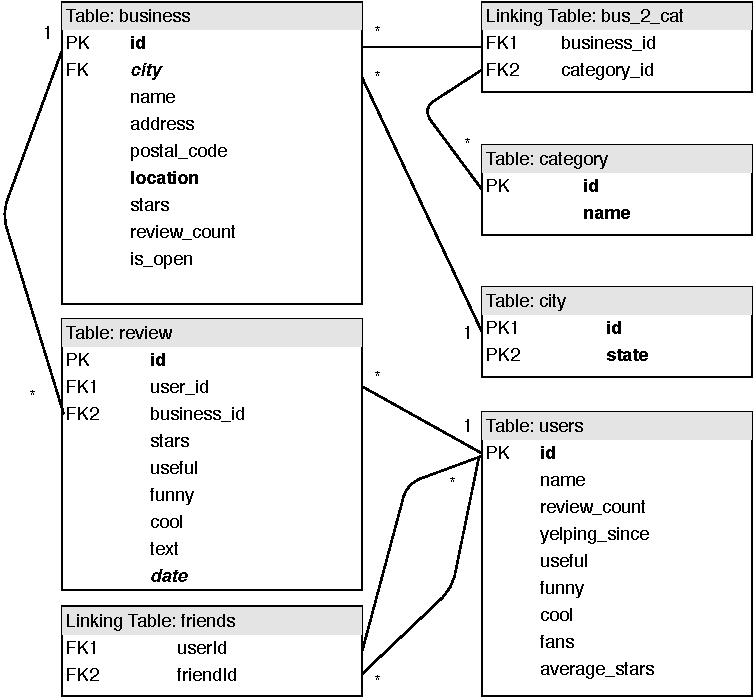
\includegraphics[width=10cm]{img/relational-design.pdf}
    \caption{A UML diagram of the relational design of the Yelp dataset. Indexed attributes are in bold whereas clustered attributes are in italics.}
    \label{fig:relational-design}
\end{figure*}

A business category and a user's friends are many-to-many relationships. The linking tables \texttt{bus\_2\_cat} and \texttt{friends} tables handle these relationships.

\subsubsection{Graph Design}

The JanusGraph design can be seen in Figure \ref{fig:janusgraph-design} whereas the TigerGraph design can be see in Figure \ref{fig:tigergraph-design}. The motivation for the difference in the two designs is mainly due to the graphs handling spatial data differently.

JanusGraph indexes attributes on nodes and edges using either composite indexes \cite{janusgraph-comp-index}, which index native data types on equality conditions, or mixed indexes which leverages an indexing backend on more complex data types or for complex search predicates, e.g. fuzzy search on strings \cite{janusgraph-mixed-index}.

Figure \ref{fig:janusgraph-design} show which attributes are indexed using composite indexes and which use mixed indexes -- making use of the indexing backend. As in Section \ref{subsub:relational-design}, \emph{location} is indexed using R-trees with ElasticSearch's geo-search predicates. \emph{Date} is indexed using ElasticSearch for equality conditions using the \texttt{java.time.Instant} class -- this uses a Bkd-tree indexing implementation \cite{es-bkdtree-index}.

\begin{figure*}[h]
    \centering
    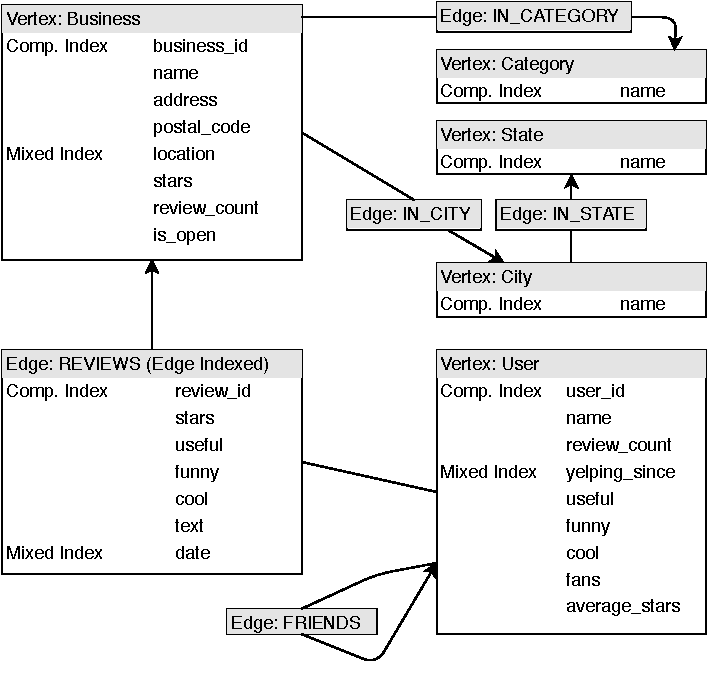
\includegraphics[width=10cm]{img/janus-design.pdf}
    \caption{A UML diagram of the graph design for JanusGraph.}
    \label{fig:janusgraph-design}
\end{figure*}

TigerGraph puts less of a focus on indexing and more on writing efficient and fast queries. One notable difference between the structure in the JanusGraph implementation and the TigerGraph implementation in Figure \ref{fig:tigergraph-design} is that there are no indexes and the extension of the \emph{location} attribute as the \texttt{Business\_Geo} edge and \texttt{Geo\_Grid} vertex. The code leveraged for this design idea was inspired from the TigerGraph geospatial webinar \cite{graphgurus} and C++ code on the TigerGraph ```ecosys''\footnote{\url{https://github.com/tigergraph/ecosys/tree/master/guru\_scripts/geospatial\_search}}.

\begin{figure*}[h]
    \centering
    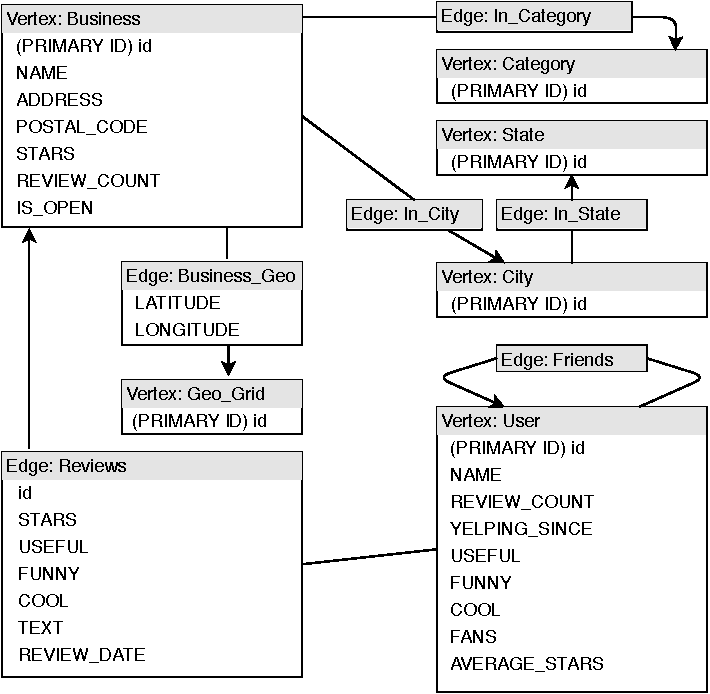
\includegraphics[width=10cm]{img/tigergraph-design.pdf}
    \caption{A UML diagram of the graph design for TigerGraph.}
    \label{fig:tigergraph-design}
\end{figure*}

